%%%%%%%%%%%%%%%%%%%%%%% CHAPTER - 3 %%%%%%%%%%%%%%%%%%%%\\
\chapter{Methodology Adopted}
\label{C3} %%%%%%%%%%%%%%%%%%%%%%%%%%%%
%\noindent\rule{\linewidth}{2pt}
%%%%%%%%%%%%%%%%%%%%%%%%%%%%%%%%%%%%%%%%%%%%%%%%%%%%%%%%%
\section{Algorithms}

% \begin{equation}
% \label{eq1}
%     (a+b)^2=(a)^2+(b)^2
% \end{equation}

% where, $a$, and $b$ are the variables.

\subsection{Training Algorithm -}
    \begin{algorithmic}[1]
        \item \textit{Extract the text from the document.}
        \item \textit{Tokenize the data.}
        \item \textit{Preprocess the data -}
        \begin{itemize}
            \item \textit{Remove whitespaces}
            \item \textit{Remove any digit in between square brackets.}
            \item \textit{Remove Stop words.}
        \end{itemize}
        \item \textit{Tag the data.}
        \item \textit{Train a model using the tagged data.}
        \item \textit{Store the trained model.}
        \item \textit{Stop.}
    \end{algorithmic}
    
\subsection{Vectorization Algorithm -}
    \begin{algorithmic}[1]
        \item \textit{Extract the text from the original answer script and the sample answer script.}
        \item \textit{Tokenize the data.}
        \item \textit{Preprocess the data -}
        \begin{itemize}
            \item \textit{Remove whitespaces}
            \item \textit{Remove any digit in between square brackets.}
            \item \textit{Remove Stop words.}
        \end{itemize}
        \item \textit{Vectorize the text using the pre-trained model.}
        \item \textit{Store the vectors.}
        \item \textit{Stop}
    \end{algorithmic}
    
\subsection{Clustering Algorithm -}
\begin{algorithmic}[1]
    \State \textit{Cluster all the vectors except the Sample answer vector.}
    \If{Vector is in a Cluster}
        \State \textit{Store the Cluster number and the vector;}
        \State \textit{Go to Step 9;}
    \Else
        \State \textit{Store the vector as an Outlier;}
        \State \textit{Go to Step 20;}
    \EndIf
    \For{n in number(clusters)}
        \State \textit{Calculate the midpoint of n}
        \State \textit{Calculate the similarity between the midpoint and the sample answer vector.}
    \EndFor
    \For{n in number(clusters)}
        \For{i in points(n)}
            \State \textit{Score of i = Score of midpoint(n);}
            \State \textit{Store the similarity scores in Scores.}
        \EndFor
    
    \EndFor
    \State \textit{Go to Step 23}  % Check Plz
    \For{n in number(outliers)}
        \State \textit{Calculate the similarity score of n with the sample answer vector.}
    \EndFor
    \State \textit{Stop}

\end{algorithmic}

\subsection{Final marking Algorithm -}
\begin{algorithmic}[1]
    \State \textit{Enter full marks F for the question.}
    \For{ j in Scores}
        \State $Final\_marks \gets j \times F$
    \EndFor
    \State \textit{Display the Final\_marks.}
\end{algorithmic}

%\begin{comment}
    \newpage
% Flowchart of the methodology is shown in Figure \ref{Flowchart}.
\section{Flowchart}
   \begin{figure}[H]
       \centering
       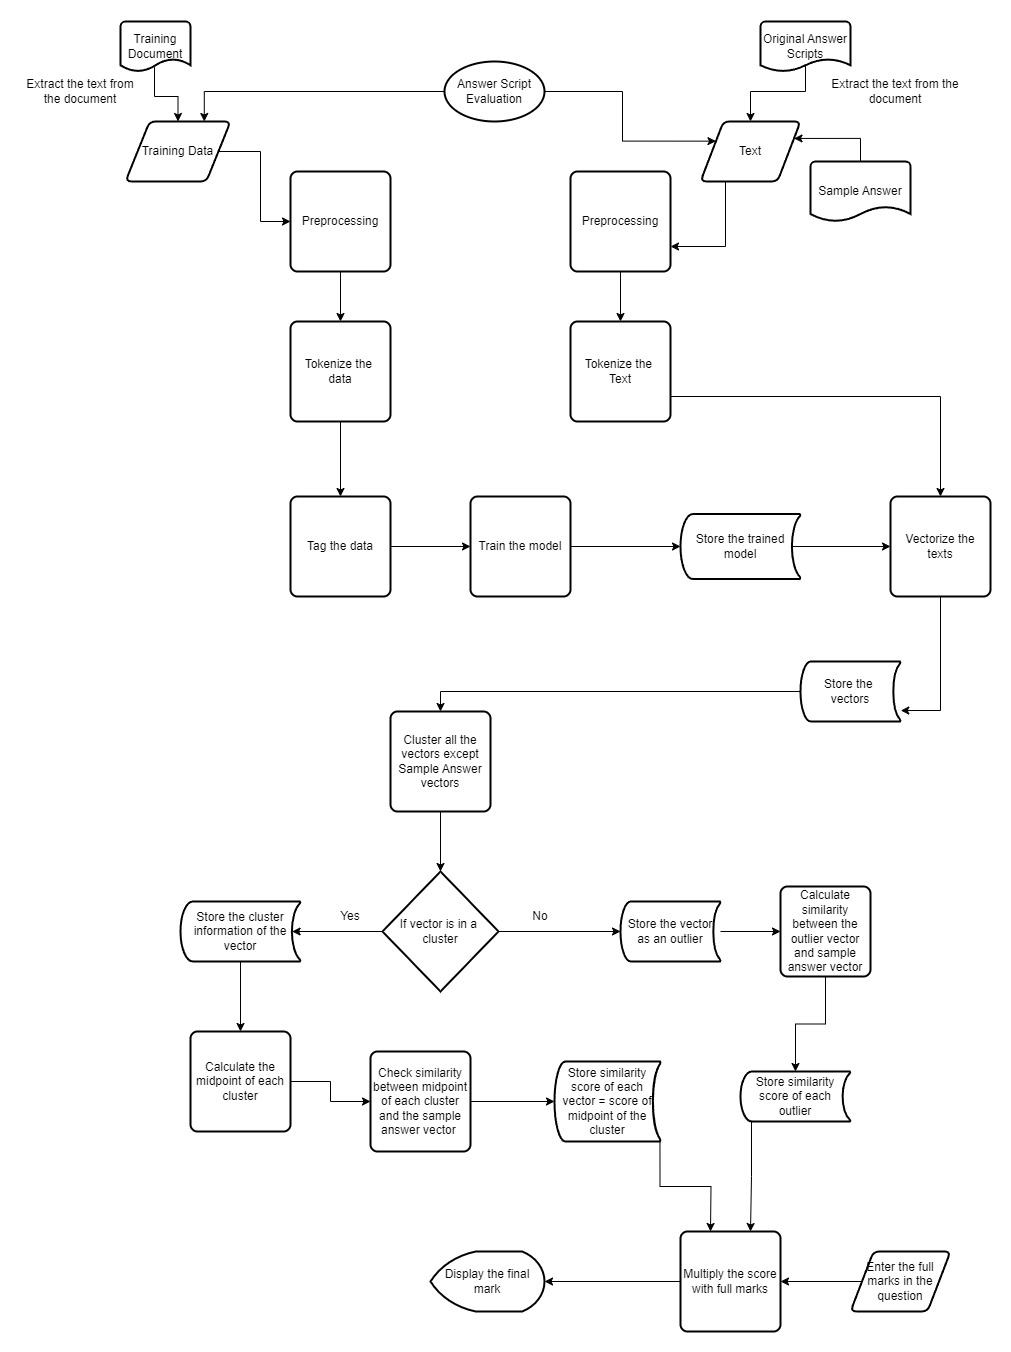
\includegraphics[width=1\linewidth]{IMAGE/flowchart.jpeg}
       \caption{Flowchart of the Methodology}
       \label{Flowchart}
   \end{figure}
%\end{comment}

\newpage
\section{Discussion}
    \par
    The automation of Answer script evaluation is a critical task. It has quite a lot of challenges like 
    understanding the literature of every answer, processing the idea behind the answer, and evaluating the 
    correctness of that idea. In this article, we are going to discuss a method by which we can overcome these 
    challenges and can automate the task. 
    \par
    This technique consists of 4 major sections. These are - 
    \begin{itemize}
        \item Training
        \item Vectorization
        \item Clustering
        \item Final marking
    \end{itemize}

%    \begin{comment}
   \begin{figure}[H]
       \centering
       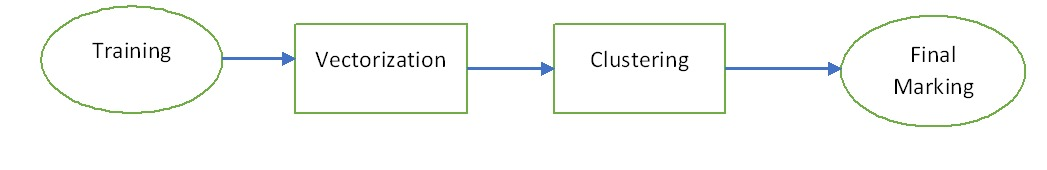
\includegraphics[width=1\linewidth]{IMAGE/steps.jpeg}
       \caption{ Process Diagram }
       \label{Steps}
   \end{figure}
%    \end{comment}
%
    \subsection{Training}
        \par
        In Machine Learning, Training is a pivotal phase. It requires additional care as it impacts on the 
        outcome of the process.  The processing of data, the selection of hyperparameters, and analysis of 
        error - these are all integral parts of efficient training of a machine learning model. In this article,
        we have discussed an Unsupervised learning technique called Word-Embeddings. This technique requires 
        training with tagged text data that will put every word in a multi-dimensional vector space. 
        This technique helps to determine how close two words are, in terms of semantic meaning. Thus for training,
        we require a text corpus that will have relevance to the topic of the exam. This corpus could be 
        supplied by any textbook or research paper on the topic.
        \par
        For training purposes, the book has to be segmented into several text files. Now, 
        a complete text consists of different unnecessary things that are used only for literature 
        purposes and have little to do with the analysis of text. Adding these to the training data 
        could lead to biased and incorrect conclusions. To avoid this, the text needs to be processed first. 
        Several natural language techniques offer efficient preprocessing of data. As part of preprocessing the 
        whitespaces in the text are removed. Then any digit within square brackets is removed. Any sequence of 
        numbers of digits is also removed. And finally, stop words are removed.
        \par
        Stop words are some extremely common words that have little value in expressing the significance of 
        certain text. Some examples of Stop Words are - 'a', 'an', 'is', 'of', 'on' etc. Removing these words 
        will not affect the training process. After the preprocessing is done, the tokenization is applied to the
        text. Tokenization is a technique where documents are chopped into pieces, which are called Tokens.
        In this process, the punctuations are also removed. After the tokenization is done, the text is ready
        to go for training.
        \par
        To train the model, we need tagged text. Document tagging is a process where each document is 
        represented with a numeric value, called Tag. Once the tagging is done, we could train the embedding model 
        using the tagged data.
    
    \subsection{Vectorization}
        \par
        In the post-training phase, the trained model is implemented on actual data. The original answer scripts 
        are passed in text format as input. Additionally, a sample answer to the questions is needed for 
        evaluation in the final phase. This sample answer file is also included as input at this stage. 
        After the files are inputted, they are to be passed through processing. We will perform the same 
        preprocessing steps as we did in the training phase:
        \begin{itemize}
            \item Remove one or more whitespaces.
            \item Remove any digit within square brackets.
            \item Remove any sequence of numbers or digits.
            \item Remove the stop words.
            \item Tokenize the text.
        \end{itemize}
        \par
        Upon completion of preprocessing, the text is prepared for vectorization. The cleaned text is passed 
        through the pre-trained model, enabling the conversion of text data into vector representations. 
        This vectorization process facilitates subsequent analysis and evaluation of the answer scripts, 
        ultimately contributing to the automated answer script evaluation system's effectiveness and accuracy.

    \subsection{Clustering}
        \par
        In the preceding step, we obtained document vectors representing numerical representations of each document. Now to determine the proximity of these vectors, we will perform clustering on them. The idea behind this clustering is to divide all the answers into a few categories so that we can evaluate the categories to determine the quality of each answer. The clustering step is quite simple. By choosing a clustering algorithm, pass all the vectors, except the sample answer vector, through it. If a vector is in a cluster, store the vector and its corresponding cluster-ID in a separate space. If the vector is not in a cluster, it would be classified as an outlier and will be stored in a different place. We do not pass the sample answer vector in the clustering model, it will be used for the final evaluation.
        \par
        After classifying all the vectors correctly between cluster member and outlier, we will proceed to the subsequent step. For the clustered vectors, we will compute the midpoints of all the clusters. Then the similarity between the midpoints and the sample answer vector is calculated. Finally, the same score for each cluster midpoint is assigned to every member of the corresponding cluster.
        \par
        In the case of outliers, we directly calculate the similarity of each one with the sample answer vector. Here, we assume that the number of outliers is lesser so that the computation takes less time. However, if the number of outliers is substantial, it may necessitate longer computation times and could potentially lead to different conclusions. Possible implications include inefficient training or the need to fine-tune clustering hyperparameters.
        \par
        By systematically applying clustering and similarity evaluation techniques, we aim to enhance the accuracy and efficiency of the automated answer script evaluation process.

    \subsection{Final marking}
        \par
        In the final evaluation step, we take the highest mark of the question as input. The similarity score that we obtained in the previous section denotes the similarity between the sample answer and the corresponding original answer. That way, the similarity score serves as a metric indicating the correctness of the specific answer. We can assume it as a percentage of how much the answer is correct.
        \par
        In the final evaluation, we leverage this similarity score by multiplying it with the full marks designated for the question. This calculation produces the final marks awarded to the answer, encapsulating both its accuracy and alignment with expected standards. By employing this approach, we aim to provide a comprehensive and equitable assessment of each answer's merit, facilitating meaningful feedback to students and enhancing the effectiveness of automated answer script evaluation.
    
        
            




